\documentclass{standalone}
\usepackage{tikz, pgfplots, xcolor}
\pgfplotsset{compat=1.18}

\definecolor{CustomB1}{RGB}{17,117,167}
\definecolor{CustomB2}{RGB}{60,84,111}

\begin{document}
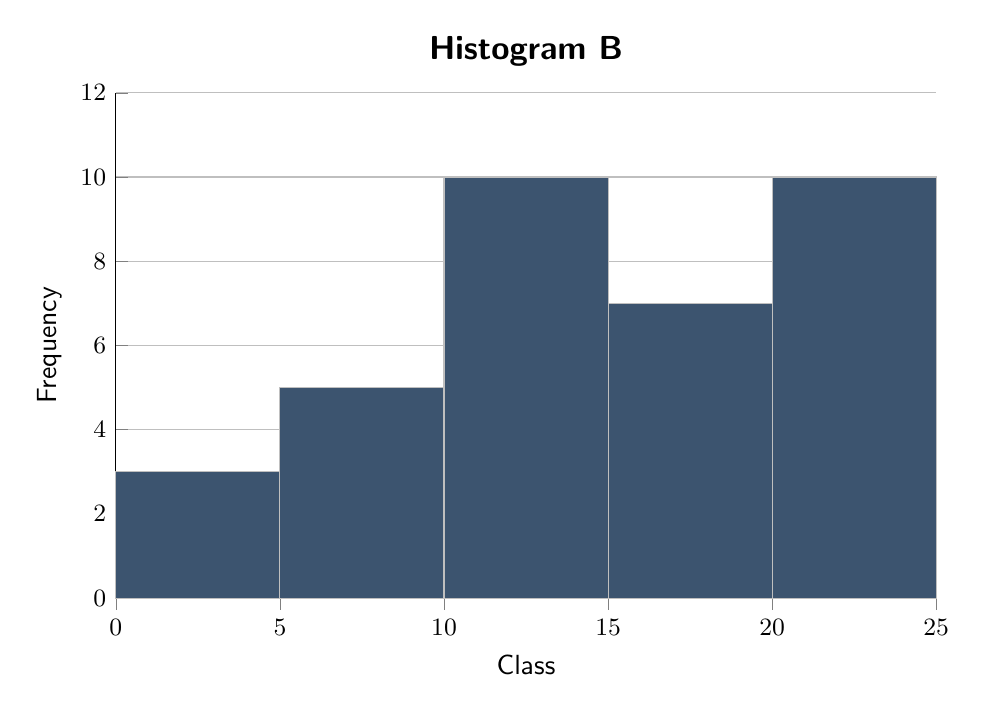
\begin{tikzpicture}
  \begin{axis}[
      xlabel style={font=\sffamily},
      ylabel style={font=\sffamily},
      ticklabel style={font=\sffamily},
      axis lines*=left,
      no markers,
      xmin=0, xmax=25, ymin=0, ymax=12,
      xtick={0,5,10,15,20,25},
      ytick={0,2,...,12},
      xlabel={Class},
      ylabel={Frequency},
      title={\large\bfseries\sffamily Histogram B},
      ticklabel style={font=\small},
      enlargelimits=false,
      clip=false,
      grid = none,
      ymajorgrids=true,
      ybar=0pt,
      width=12cm,
      height=8cm
    ]
    \addplot+[ybar interval, fill=CustomB2, draw=lightgray] plot coordinates {
        (0, 3)
        (5, 5)
        (10, 10)
        (15, 7)
        (20, 10)
        (25,0)
    };
  \end{axis}
\end{tikzpicture}
\end{document}